\documentclass[12pt]{article}
% \usepackage[brazilian]{babel}
\usepackage[a4paper,inner=1.5cm,outer=1.5cm, total={6in, 8in}]{geometry}
\usepackage[utf8]{inputenc}
\usepackage{lmodern}
\usepackage{graphicx}
\usepackage{float}
\usepackage{newtxmath}
\usepackage{amssymb, amsmath, amsfonts, array}
\usepackage{bm}
\usepackage{indentfirst}

\title{TIP8419 - Tensor Algebra\\ 
       Homework 1}
\author{Ezequias Márcio - $497779$}
\date{\today}

\begin{document}

\maketitle

\section*{Kronecker Product}\vspace{.5cm}

\noindent
\textbf{Problem 1.} For randomly generated matrices 
$\bm{A} \in \mathbb{C}^{N\times N}$ and $\bm{B}\in \mathbb{C}^{N\times N}$, 
evaluate the computational performance (run time) of the following matrix 
inversion formulas: 

\begin{itemize}
    \item [(a)] Method 1: $(\bm{A}_{N\times N}\otimes \bm{B}_{N\times N})^{-1}$
          
    Method 2: $\bm{A}^{-1}_{N\times N}\otimes \bm{B}^{-1}_{N\times N}$
    
    for $N \in \{2,4,8,16,32,64\}$.\\

    \item [(b)] Method 1: $(\bm{A}^{(1)}_{4\times 4}\otimes 
    \bm{A}^{(2)}_{4\times 4} \otimes ...\otimes 
    \bm{A}^{(K)}_{4\times 4})^{-1} = \bigg(\bigotimes\limits^{K}_{i = 1}
    \bm{A}^{(i)}_{4\times 4}\bigg)^{-1}$\\

    Method 2: $(\bm{A}^{(1)})^{-1}_{4\times 4}\otimes 
    (\bm{A}^{(2)})^{-1}_{4\times 4}\otimes ...\otimes 
    (\bm{A}^{(K)})^{-1}_{4\times 4} =\bigotimes\limits^{K}_{i = 1} 
    (\bm{A^{(i)}})^{-1}_{4\times 4}$

    for $K \in \{2,4,6,8,10\}$.

\end{itemize}

\noindent \textbf{Solution:}\\

%------------------------------------------------------------------------------
The algorithm used to calculate the Kronecker product in this work was 
implemented in \texttt{python} and it can be found in the file 
\texttt{tensoralg.py}. The run time curves are result of a Monte Carlo 
simulation with $100$ realizations that was implemented in the file 
\texttt{hw1\_presentation.ipynb}.

\begin{itemize}
    \item [(a)] In Figure \ref{invkron}, we can see the 
difference of execution time between the two strategies to calculate the 
Kronecker product inversion from the logarithmic scale plot. With the growth 
of the number of columns/rows $N$, Method $2$ (blue curve) presented a better 
performance as expected, because is more computationally expensive 
to compute a matrix inversion of a large matrix e.g. 
$(\bm{A} \otimes \bm{B})_{n^2 \times n^2 }$, that have a computational complexity 
proportional to the cube of the matrix size $(n^4)^3$, than do the Kronecker product 
between the two inverses 
$\bm{A}^{-1}_{n\times n} \otimes \bm{B}^{-1}_{n\times n}$ that only requires 
$n^4$ multipications plus the cost to compute each matrix inversion. 

\begin{figure}[!ht]
    \centering 
    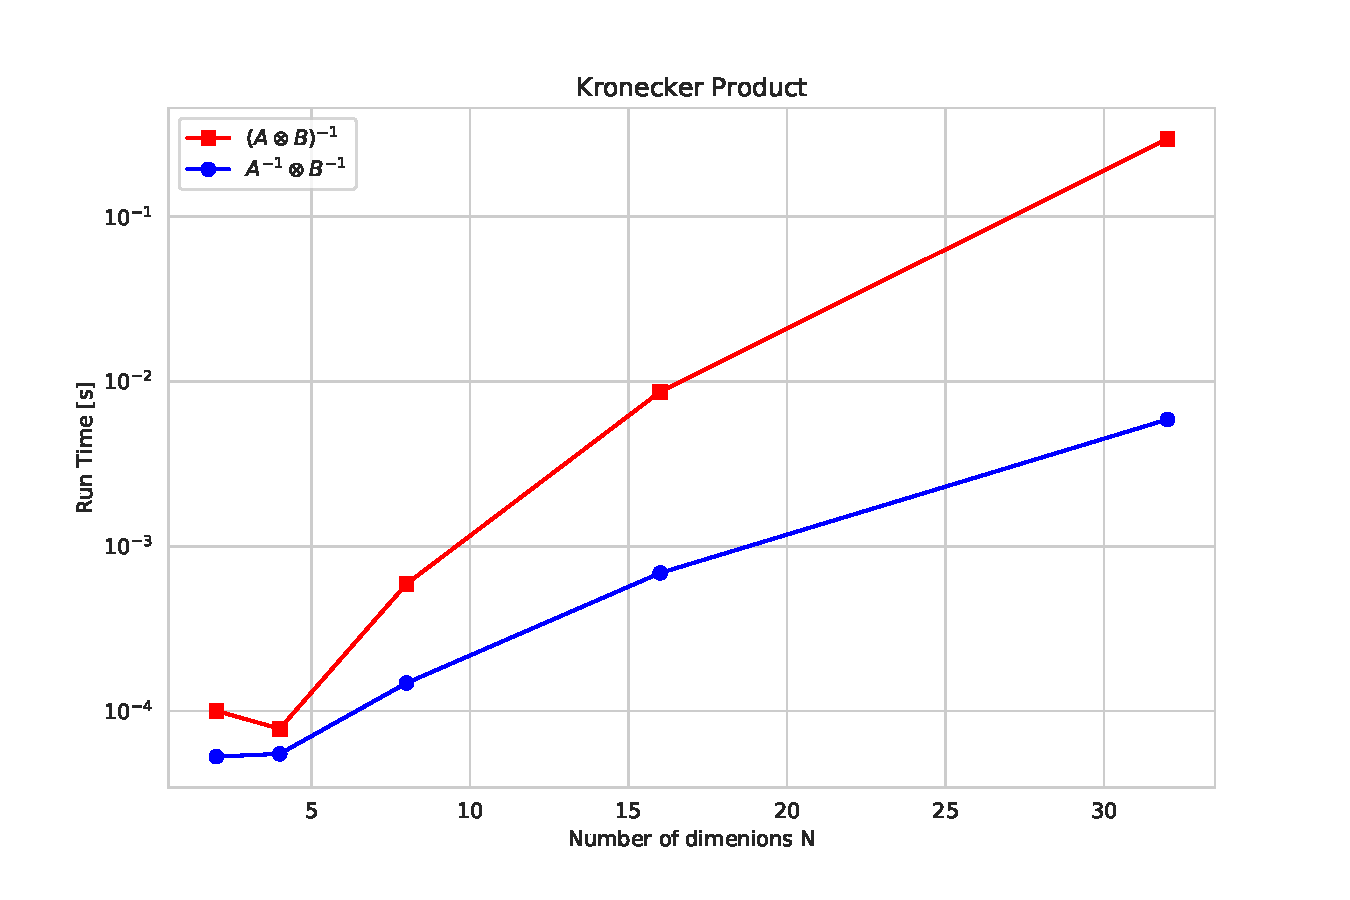
\includegraphics[width=0.65\linewidth]{figs/invkron.pdf}
    \caption{Comparsion of Kronecker product inversion formulas.}
    \label{invkron}
\end{figure}

    \item [(b)] In Figure \ref{nkron}, we can see again the computational gain 
provided by routines that calculates the matrix inversion before the Kronecker 
product. Here, Method $1$ (red curve) costs more time to compute the nested 
product once that the size of the matrix resulting from the k-th Kronecker 
product is taken into account to the complexity of the matrix inversion.

\begin{figure}[H]
    \centering 
    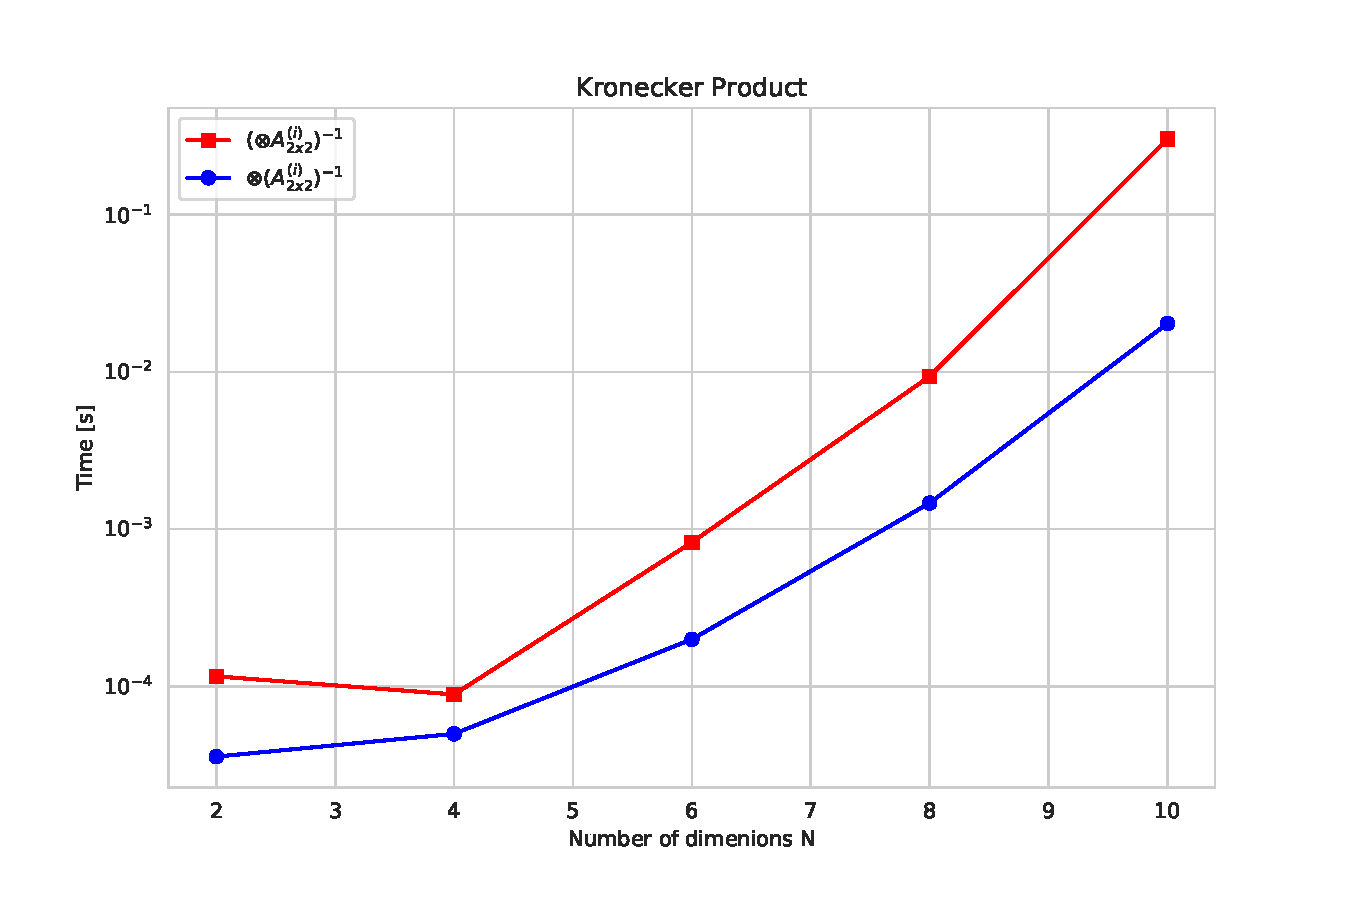
\includegraphics[width=0.65\linewidth]{figs/ninvkron.pdf}
    \caption{Comparsion of nested Kronecker product inversions.}
    \label{nkron}
\end{figure}

\end{itemize}
%------------------------------------------------------------------------------

\noindent
\textbf{Problem 2.} Let $\text{eig} (\bm{X})$ be the function that returns the 
matrix $\sum_{K\times K}$ of eigenvalues of $\bm{X}$. Show algebraically that 
$\text{eig}(\bm{A}\otimes\bm{B}) = 
\text{eig}(\bm{A})\otimes\text{eig}(\bm{B})$.\\

\noindent \textbf{Solution:}\\

%------------------------------------------------------------------------------
First, from the SVD of the matrices $\bm{A}$ and $\bm{B}$ we have:
\begin{align*}
    \bm{A} &= \bm{U}_1 \bm{\Sigma}_1 \bm{V}_{1}^{H}\\
    \bm{B} &= \bm{U}_2 \bm{\Sigma}_2 \bm{V}_{2}^{H},
\end{align*}
then, applying these definitions to the equation 
$\text{eig}(\bm{A}\otimes\bm{B})$ and using the property 
$(A\otimes B)(C\otimes D) = AC\otimes BD$ two times we have:
\begin{align*}
    \text{eig}\big(\bm{U}_1 \bm{\Sigma}_1 \bm{V}_{1}^{H}\otimes 
    \bm{U}_2 \bm{\Sigma}_2 \bm{V}_{2}^{H}\big) &=
    \text{eig}\big\{ \big( \bm{U}_1 \otimes \bm{U}_2 \big)
    \big( \bm{\Sigma}_1 \bm{V}_{1}^{H} \otimes \bm{\Sigma}_2 \bm{V}_{2}^{H}\big)
    \big\}\\
        &= \text{eig}\big\{ \big( \bm{U}_1 \otimes \bm{U}_2 \big)
        \big( \bm{\Sigma}_1 \otimes \bm{\Sigma}_2 \big)
        \big( \bm{V}_{1} \otimes \bm{V}_{2}\big)^{H}\big\}\\
        &= \bm{\Sigma}_1 \otimes \bm{\Sigma}_2 = 
        \text{eig}\big( \bm{A}\big) \otimes \text{eig}\big( \bm{B} \big),
\end{align*} by applying the operator $\text{eig}(\cdot)$ that returns the 
eigenvalue matrix $\bm{\Sigma}_1 \otimes \bm{\Sigma}_2$. 

%------------------------------------------------------------------------------

\end{document}
